\documentclass{vilniustech}
\vilniustechsetup{
    university={Vilniaus Gedimino technikos universitetas},
    faculty={Fundamentinių mokslų fakultetas},
    cathedral={Informacinių sistemų katedra},
    workTitle={Informacinių technologijų saugos metodai},
    workType={Praktinis darbas nr. 2 - Saugi WEB autentifikacija},
    workAuthorGroup={ITSfm-22},
    workAuthorNames={Aurimas Šakalys\\Aleksandr Prišmont\\Vytautas Rastenis},
    workRecipient={lektorius Vitalijus Gurčinas }
}
\addbibresource{hw1.bib}
\VTDocumentBegin

\section{Santrumpos}

\begin{itemize}
    \item \textit{TLS - Transport Layer Security};
    \item \textit{SSL - Secure Socket Layers};
    \item \textit{SAN - Subject Alternate Name};
    \item \textit{CA - Certificate Authority};
    \item \textit{CSR - Certificate Signing Request};
    \item \textit{JSON - JavaScript Object Notation};
    \item \textit{2FA - Two Factor Authentication}.
\end{itemize}

\section{Įvadas}

Šio darbo tema - realizuoti \textit{TLS/SSL} autentikaciją ir papildomą mechanizmą. Darbe formuluojami papildomi uždaviniai, norint gauti maksimalų balą:

\begin{enumerate}
    \item Įgyvendinti atsarginį autentikacijos sprendimą;
    \item Atstatyti vartotojo kredencialus;
    \item Centralizuotas vartotojų prisijungimo duomenų panaikinimas arba atstatymas.
\end{enumerate}

\section{Kas yra \textit{TLS/SSL}?}
\textit{TLS} \parencite{rescorla2018transport} (anksčiau žinomas kaip \textit{SSL} \parencite{freier2011secure}) - kriptografinis protokolas, leidžiantis saugų duomenų apsikeitimą tarp interneto mazgų. \textit{TLS} naudoja tiek simetrinį, tiek asimetrinį šifravimą. Kadangi asimetrinis šifravimas reikalauja daugiau resursų, nei simetrinis, asimetrinis šifravimas \textit{TLS}  protokole naudojamas apsikeisti simetrinio šifravimo raktu. 

\textit{TLS} protokole yra naudojami sertifikatai, kurie gali atlikti kelias funkcijas, kaip identifikavimas, viešojo ar privataus rakto laikmena. \textit{TLS} sertifikatai skirstomi į kategorijas pagal apimamą domenų sritį:

\begin{enumerate}
    \item Vieną domeną apimantis - \textit{SSL} sertifikatas;
    \item Apimantis daugiau nei vieną domeną/subdomeną - \textit{SSL SAN} sertifikatas;
    \item Apimantis visus domeno subdomenus - \textit{SSL Wildcard} sertifikatas;
\end{enumerate}

\subsection{Kas yra \textit{CA}?}
\textit{CA} \parencite{housley1999rfc2459} yra institucija, kuri tvirtina ir išduoda skaitmeninius sertifikatus, skirtus identifikuoti tam tikrus subjektus, kaip tinklalapius, el. pašto adresus, juridinius ar fizinius subjektus.

\subsection{Kaip vykdomas sertifikato patvirtinimas?} \label{sec:csr}
Norint gauti skaitmeninį sertifikatą valdomam subjektui, tai galima atlikti keliais būdais. Vienas jų - sertifikatą sugeneruoti ir patvirtinti pačiam. Tokiu būdu, sau išduotas sertifikatas suteikia visas kriptografines funkcijas, kaip \textit{CA} pasirašytas sertifikatas. Pagrindinis skirtumas tas, jog jungiantis į interneto mazgą, kuris naudoja pačio pasirašytą \textit{SSL} sertifikatą, mums bus patarta, jog sertifikatas nėra pasirašytas \textit{CA} ir užmegzti ryšį su šio mazgu gali būti pavojinga. Taip yra todėl, kad sertifikatų grandinė baigiasi \textit{CA}, kuris nėra įtrauktas į globalius patikimų \textit{CA} sąrašus.

\begin{figure}[H]
\begin{center}
    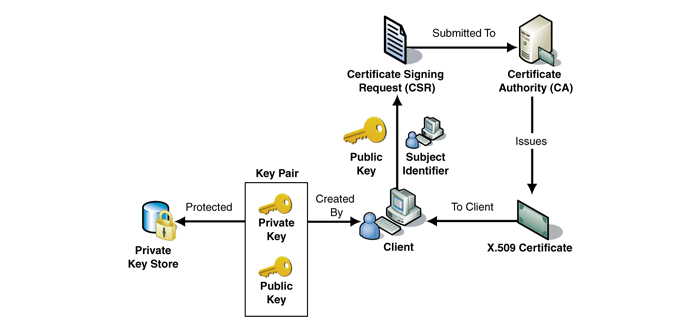
\includegraphics[height=7cm]{img/csr.png}
    \caption{\textit{CSR} pasirašymo diagrama}
    \label{fig:csr}
\end{center}
\end{figure}

Norint, kad sugeneruotą sertifikatą pasirašytų \textit{CA}, mums reikia sugeneruoti \textit{CSR} sertifikatą, ir šį pateikti \textit{CA}. \textit{CA} turintis \textit{CSR} sertifikatą, gali pasirašyti jį naudojant jų privatų raktą ir šį sertifikatą pateikti užsakovui. Šiuo atveju, jei bandoma užmegzti ryšį su mazgu, naudojančiu \textit{CA} pasirašytų sertifikatu, ryšys bus užmegztas automatiškai, asimetrinio šifravimo pagalba apsikeista simetrinio šifravimo raktais, ir simetrinio šifravimo raktų pagalba, užmegztas ryšys paverčiamas saugiu.

\section{Darbo užduoties įgyvendinimas}

Užduotis įgyvendinta sukuriant tris posistemes: \textit{CA}, serveris ir klientas.

\subsection{\textit{CA} atsakomybės}
\textit{CA} posistemė yra atsakinga už didžiąją dalį sistemos funkcionalumo. Visa komunikacija su \textit{CA} posistemiu yra atliekama naudojant \textit{HTTP RESTful API}.

\begin{figure}[H]
\begin{center}
    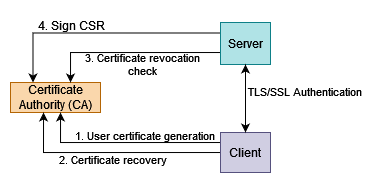
\includegraphics[height=5cm]{img/diagram.core.png}
    \caption{Bendro sistemos vaizdo diagrama}
    \label{fig:core}
\end{center}
\end{figure}

\subsubsection{Vartotojų sertifikatų generavimas} \label{section:cert_gen}

Ši funkcija yra atsakinga už sertifikatų generavimą vartotojams. Vartotojas \textit{/generate} resursui išsiunčia \textit{POST} užklausą, pateikdamas norimo subjekto vardą \parenreflst{lst:gen_post_req}. Jei šis vardas jau yra užimtas, vartotojui pateikiamas atitinkamas klaidos pranešimas. Jei vardas nėra užimtas, gaunamas atsakymas su sugeneruotu sertifikatu \textit{cert\_pem} \textit{JSON} lauke bei sertifikato atkūrimo kodu \textit{cert\_recovery} \textit{JSON} lauke \parenreflst{lst:gen_post_res}.

\begin{lstlisting}[caption=Vartotojo sertifikato generavimo JSON užklausa,label={lst:gen_post_req},language=json]
{
    "subject": "DidysisChungusas"
}
\end{lstlisting}

\begin{lstlisting}[caption=Vartotojo sertifikato generavimo JSON atsakymas,label={lst:gen_post_res},language=json]
{
    "cert_pem": "-----BEGIN CERTIFICATE-----...",
    "cert_recovery": "1Nxp..."
}
\end{lstlisting}

\subsubsection{Vartotojų sertifikatų atkūrimas}

Ši funkcija atsakingą už vartotojų sertifikatų atkūrimą, naudojant sugeneruota sertifikato atkūrimo kodą \parenrefsec{section:cert_gen}. Vartotojas \textit{/recover} resursui išsiunčia \textit{POST} užklausą, pateikdamas subjekto vardą ir atkūrimo raktą \parenreflst{lst:rec_post_req}. Jei atkūrimo raktas jau buvo panaudotas, ar atkūrimo raktas nėra skirtas nurodytam subjektui, vartotojui pateikiamas atitinkamas klaidos pranešimas. Jei pateikti duomenys yra teisingi, gaunamas atsakymas su sugeneruotu sertifikatu \textit{cert\_pem} \textit{JSON} lauke bei sertifikato atkūrimo kodu \textit{cert\_recovery} \textit{JSON} lauke \parenreflst{lst:rec_post_res}.

\textit{CA} serveris gavęs neklaidingus duomenis, jau išduotą sertifikatą paverčia negaliojančiu ir vartotojui sugeneruoja naują. Kadangi išduoti sertifikatai negali būti modifikuojami, sertifikato galiojimo nutraukimas yra įgyvendinamas įrašant sertifikatą į nebegaliojančių sertifikatų sąrašą.

Atkuriant sertifikatą, būtinybė pateikti subjekto pavadinimą padidina atkūrimo saugą. Jei \textit{blogiečiai} sužino tik atkūrimo kodą, negali padaryti žalos, nes nežino subjekto vardo.

\begin{lstlisting}[caption=Vartotojo sertifikato atkūrimo JSON užklausa,label={lst:rec_post_req},language=json]
{
    "subject": "DidysisChungusas",
    "key": "1Nxp..."
}
\end{lstlisting}

\begin{lstlisting}[caption=Vartotojo sertifikato atkūrimo JSON atsakymas,label={lst:rec_post_res},language=json]
{
    "cert_pem": "-----BEGIN CERTIFICATE-----...",
    "cert_recovery": "KyVP..."
}
\end{lstlisting}

\subsubsection{Sertifikato galiojimo patikrinimas}

Ši funkcija atsakingą už vartotojų sertifikatų galiojimo patikrinimą. Sertifikatų galiojimo laikas yra užkoduojamas pačiame sertifikate, tačiau jei sertifikato galiojimas buvo nutrauktas anksčiau laiko, egzistuojančių sertifikatų neįmanoma modifikuoti. Dėl šios priežasties, galiojimo nutraukimui \textit{CA} duomenų bazėje saugo nebegaliojančių sertifikatų sąrašą.

Vartotojas \textit{/revoked} resursui išsiunčia \textit{POST} užklausą, pateikdamas tikrinamą sertifikatą \parenreflst{lst:rev_post_req}. Priklausomai nuo sertifikato galiojimo, gaunamas atitinkamas atsakas \parenreflst{lst:rev_post_res}.

Galiojimo patikrinimas sistemos įgyvendinime vykdomas \textit{CA} serverio pusėje. Yra galimybė perduoti šį patikrinimą, autentikaciją validuojančiam serveriui, pateikiant nebegaliojančių sertifikatų sąrašą. Šio metodo trūkumas, kad galimai būtų siunčiamas didelis kiekis duomenų, taip pat autentikuojantis serveris gali klaidingai nustatyti, ar sertifikatas jau nebėra galiojantis.

\begin{lstlisting}[caption=Vartotojo sertifikato galiojimo patikrinimo JSON užklausa,label={lst:rev_post_req},language=json]
{
    "certificate": "-----BEGIN CERTIFICATE-----..."
}
\end{lstlisting}

\begin{lstlisting}[caption=Vartotojo sertifikato galiojimo patikrinimo JSON atsakymas,label={lst:rev_post_res},language=json]
{
    "revoked": false
}
\end{lstlisting}

\subsubsection{Sertifikato pasirašymas}

Ši funkcija atsakingą už serverio sertifikatų pasirašymą. \textit{CA} serveris atlieka \ref{sec:csr} skyriuje aptartą \textit{CSR} pasirašymo mechanizmą. Sertifikatas pasirašomas tik \textit{SSL} ir \textit{SSL SAN} sertifikatams, norint užtikrinti, kad autentikuojantys serveriai negalėtų apsimesti vienas kitu.

Vartotojas \textit{/sign} resursui išsiunčia \textit{POST} užklausą, pateikdamas \textit{CSR} sertifikatą \parenreflst{lst:csr_post_req}. Jei \textit{CSR} sertifikate pateikiami netinkami duomenys, vartotojui pateikiamas atitinkamas klaidos pranešimas. Jei \textit{CSR} sertifikatas yra tvarkingas, serveris gauna pasirašytą sertifikatą  \textit{cert\_pem} \textit{JSON} lauke \parenreflst{lst:csr_post_res}.

\begin{lstlisting}[caption=Serverio sertifikato pasirašymo JSON užklausa,label={lst:csr_post_req},language=json]
{
    "certificate": "-----BEGIN CERTIFICATE-----..."
}
\end{lstlisting}

\begin{lstlisting}[caption=Serverio sertifikato pasirašymo JSON atsakymas,label={lst:csr_post_res},language=json]
{
    "cert_pem": "-----BEGIN CERTIFICATE-----..."
}
\end{lstlisting}

\subsection{Serverio ir kliento autentikacija}

Klientas, jungdamasis prie serverio inicijuoja įprastą \textit{TLS} ryšį. Iš serverio gaunamas \textit{CA} pasirašytas sertifikatas \parenreflst{lst:csr_post_res}, kurį klientas gali validuoti naudojantis \textit{CA} serverio sertifikatu. Jei serverio sertifikatas yra tvarkingas, užmezgamas saugus \textit{TLS} ryšys ir pradedama vartotojo autentikacija. 

\begin{figure}[H]
\begin{center}
    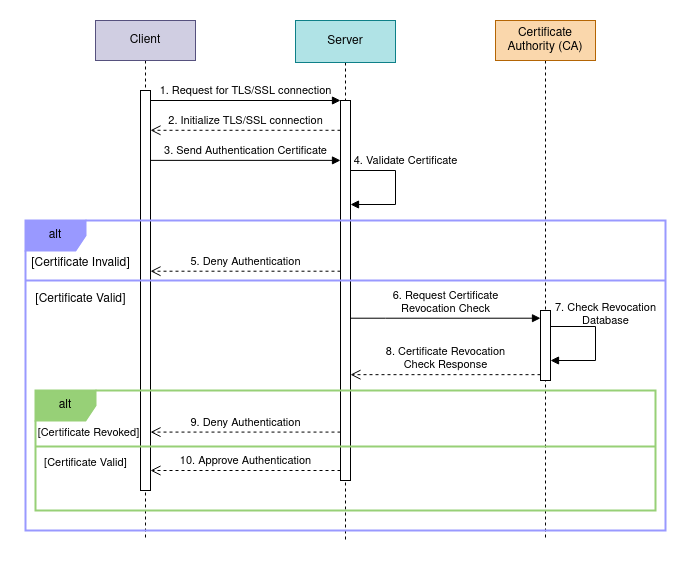
\includegraphics[height=12cm]{img/diagram.authentication.png}
    \caption{Kliento autentikavimo serveryje diagrama}
    \label{fig:core}
\end{center}
\end{figure}

Vartotojas pateikia sugeneruotą vartotojo sertifikatą \parenreflst{lst:gen_post_res}. Serveris patikrina, ar sertifikatas buvo sugeneruotas \textit{CA}, ar sertifikatas vis dar galioja. Jei patikrinimas yra nesėkmingas, vartotojo autentikavimas nutraukiamas. Kitu atveju, autentikavimas tęsiamas, serveris išsiunčia sertifikato galiojimo patikrinimo užklausą \parenreflst{lst:rev_post_req} \textit{CA} serveriui. Jei sertifikato galiojimas nutrauktas anksčiau laiko,  vartotojo autentikavimas nutraukiamas. Kitu atveju, vartotojo autentikacija baigta, vartotojas gali pasiekti serverio resursus.

\section{\textit{2FA} sprendžiamos problemos}
Nors užduoties įgyvendinime, \textit{2FA} nėra įgyvendintas, tačiau norint toliau didinti autentikacijos ir atstatymo procesų saugumą, turėtume prijungti \textit{2FA} implementaciją. Šį procesą įdiegus, autentikacijos metu padidėja saugumas - jei kažkokiu būdu kitas asmuo bando prisijungti prie sistemos, negali šio proceso užbaigti, nes neturi prieigos prie \textit{2FA} įrenginio. Taip pat padidinamas sertifikato atkūrimo saugumas, kadangi \textit{blogiečiams} gavus tiek atkūrimo kodą, tiek sertifikatą (ar tik subjektą), jie negalėtu padaryti žalos, neturint prieigos prie \textit{2FA} įrenginio.

\VTDocumentEnd